\chapter{Flux equations}
This appendix contains mathematical descriptions of all flux equations that are included in the Modular Assessment of Rainfall-Runoff Models Toolbox v2.- (MARRMoT).
For each flux equation, the mathematical constitutive function, as well as the MARRMoT code, which includes any necessary constraints, are given.
All fluxes are contained in Table \ref{tab:fluxesfunction}.

%% REFERENCES
\bibliographystyle{copernicus}
\bibliography{marrmot_model_references}

% Place a caption
\vfill{}
\captionof{table}[Computational implementation of constitutive flux equations]{Equations from model descriptions and their implementation in MARRMoT (Table starts on following page) \label{tab:fluxesfunction}}

\clearpage
\KOMAoptions{paper=A3,paper=landscape,pagesize}
\recalctypearea
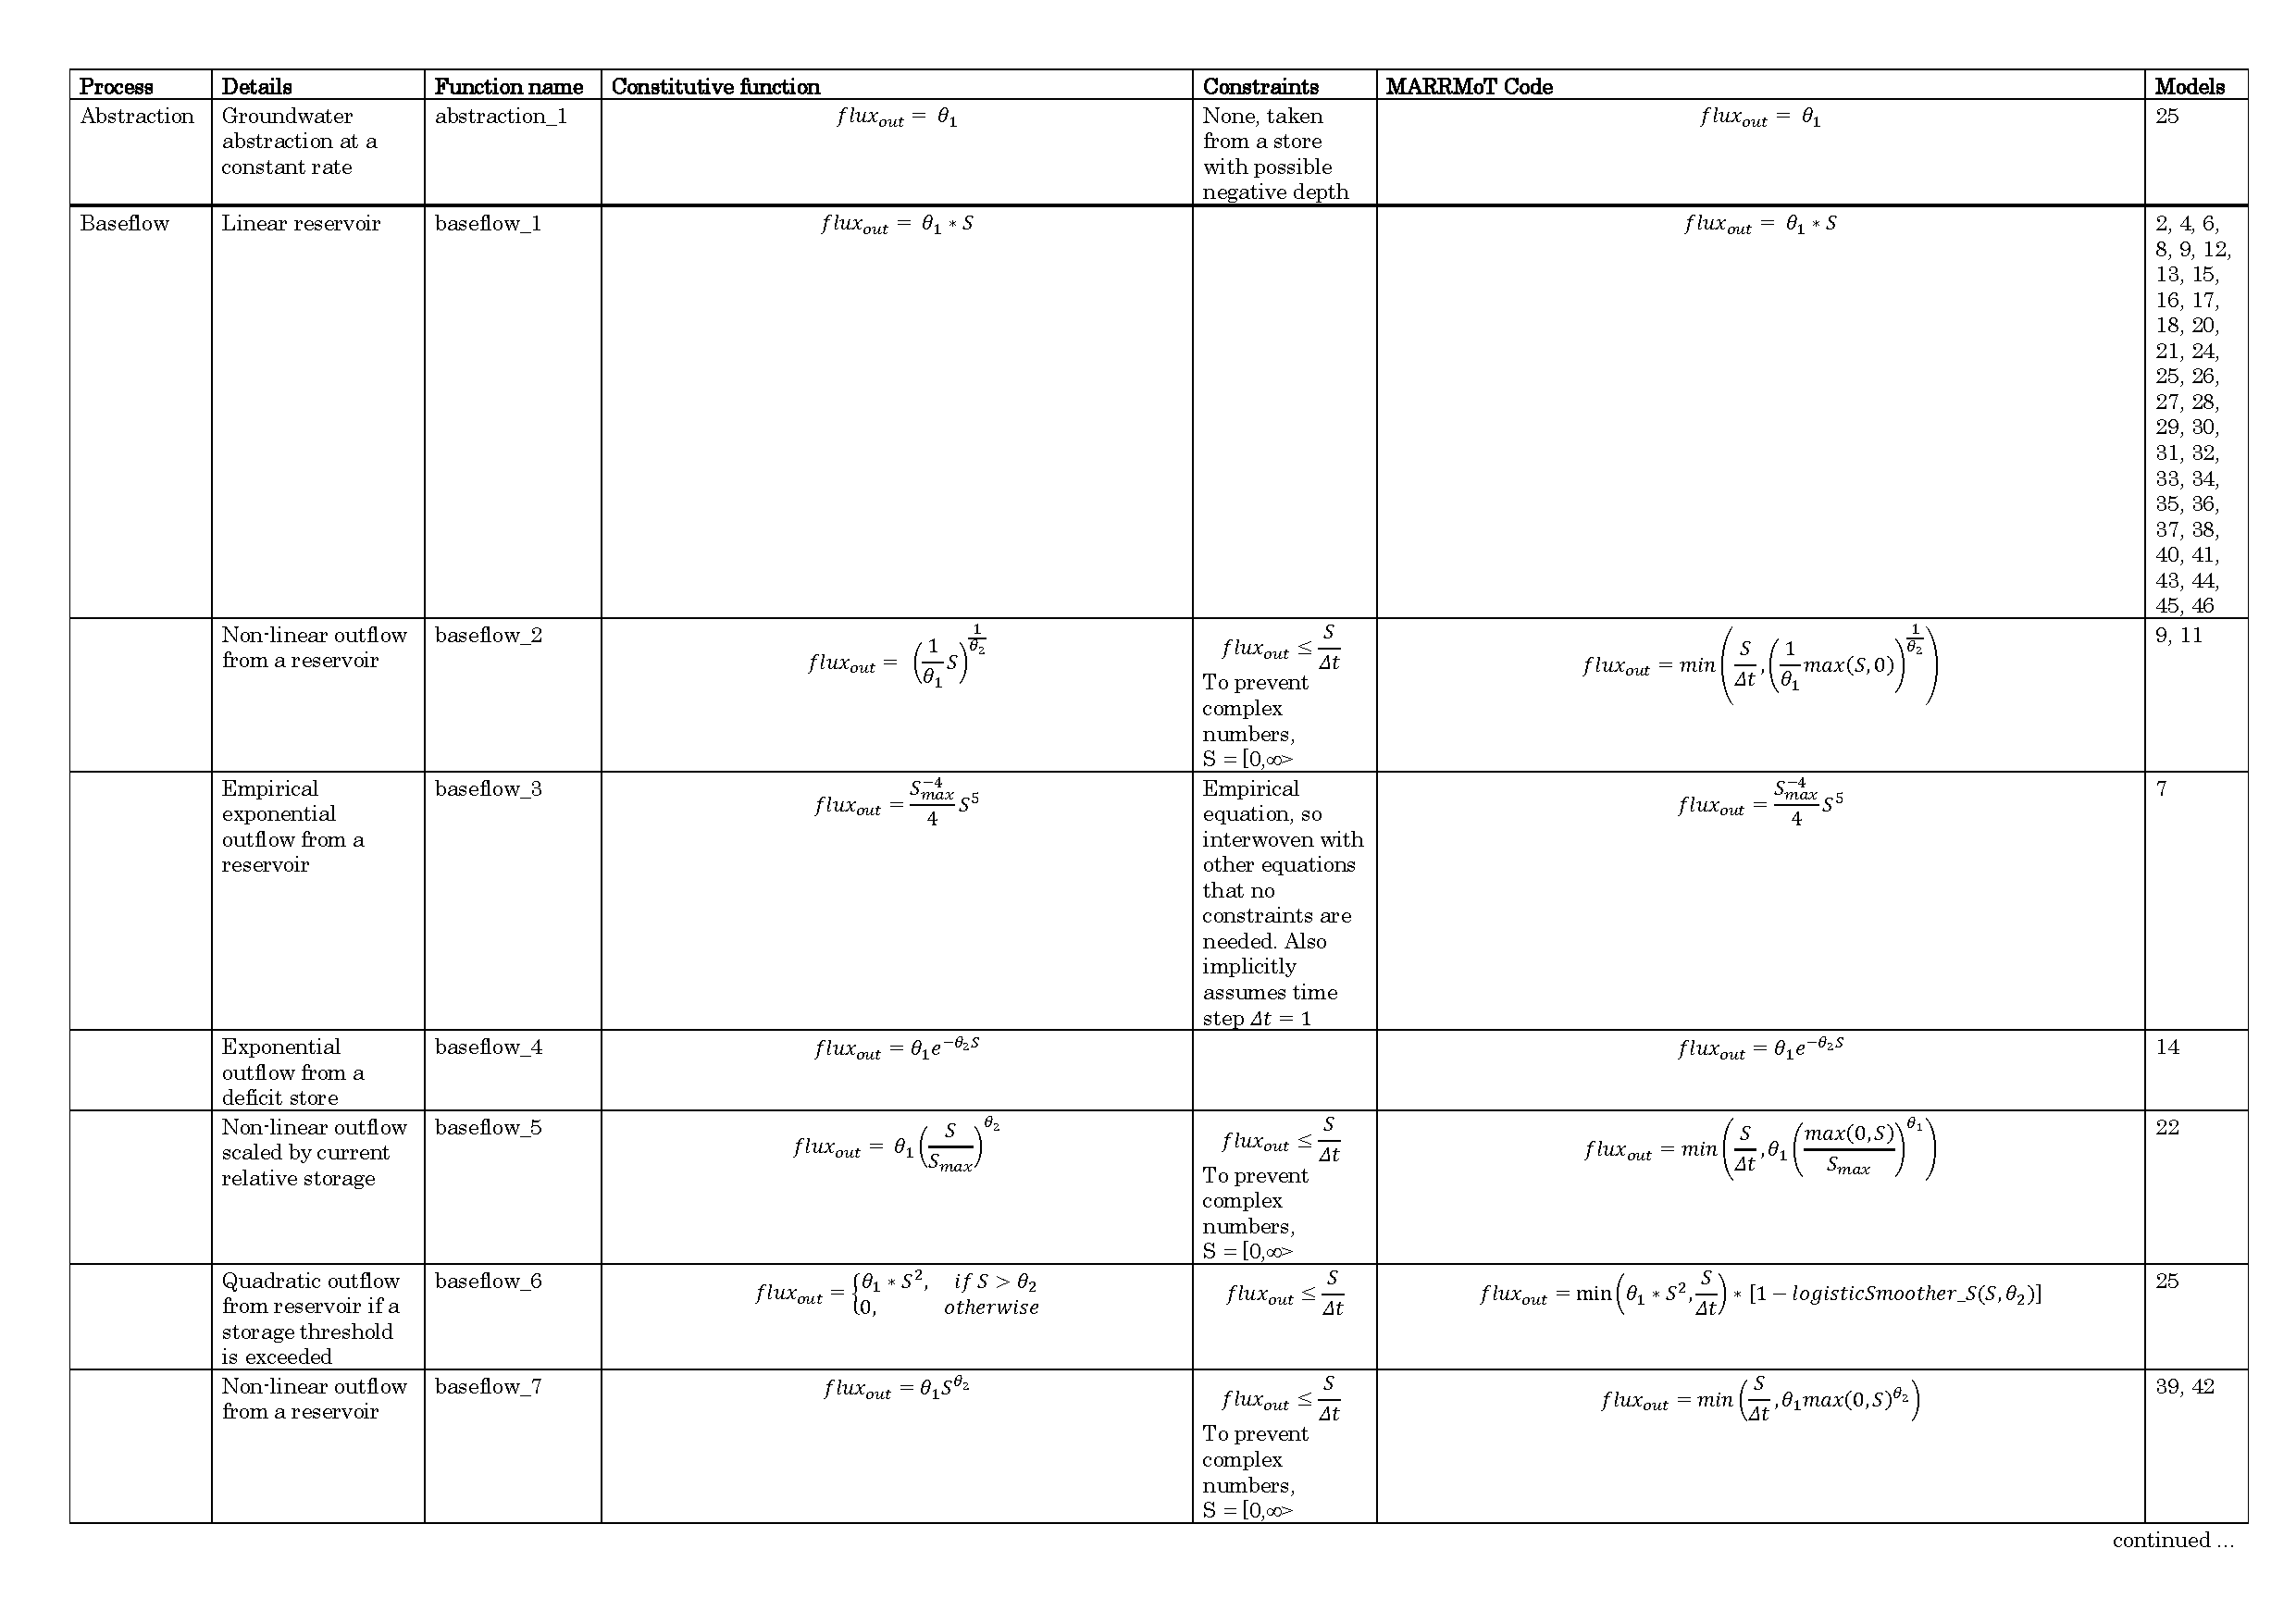
\includepdf[pages=-,pagecommand={\thispagestyle{styleLandscapeA3}}]{./AppB_files/Flux_equations_A3.pdf}

\clearpage
\KOMAoptions{paper=A4,paper=portrait,pagesize}
\recalctypearea

